\section{Implementation of Alpha}

\paragraph{}
The Alpha sketch is an improvement over the GMatrix algorithm. The idea behind the Alpha sketch is simple. It partitions the frequency matrix of the GMtrix sketch according to the partition algorithm proposed in gSketch in order to reduce the average relative error of the queries. This high-level concept of the Alpha is depicted in \autoref{fig:alpha}. The method proposed to reduce the average relative error is to recursively partition the available amount of memory according to a sample of the original graph stream. More details about the partitioning technique of gSketch will be discussed in \autoref{section:gsketch_partitioning}.

\begin{figure}[H]
    \centering 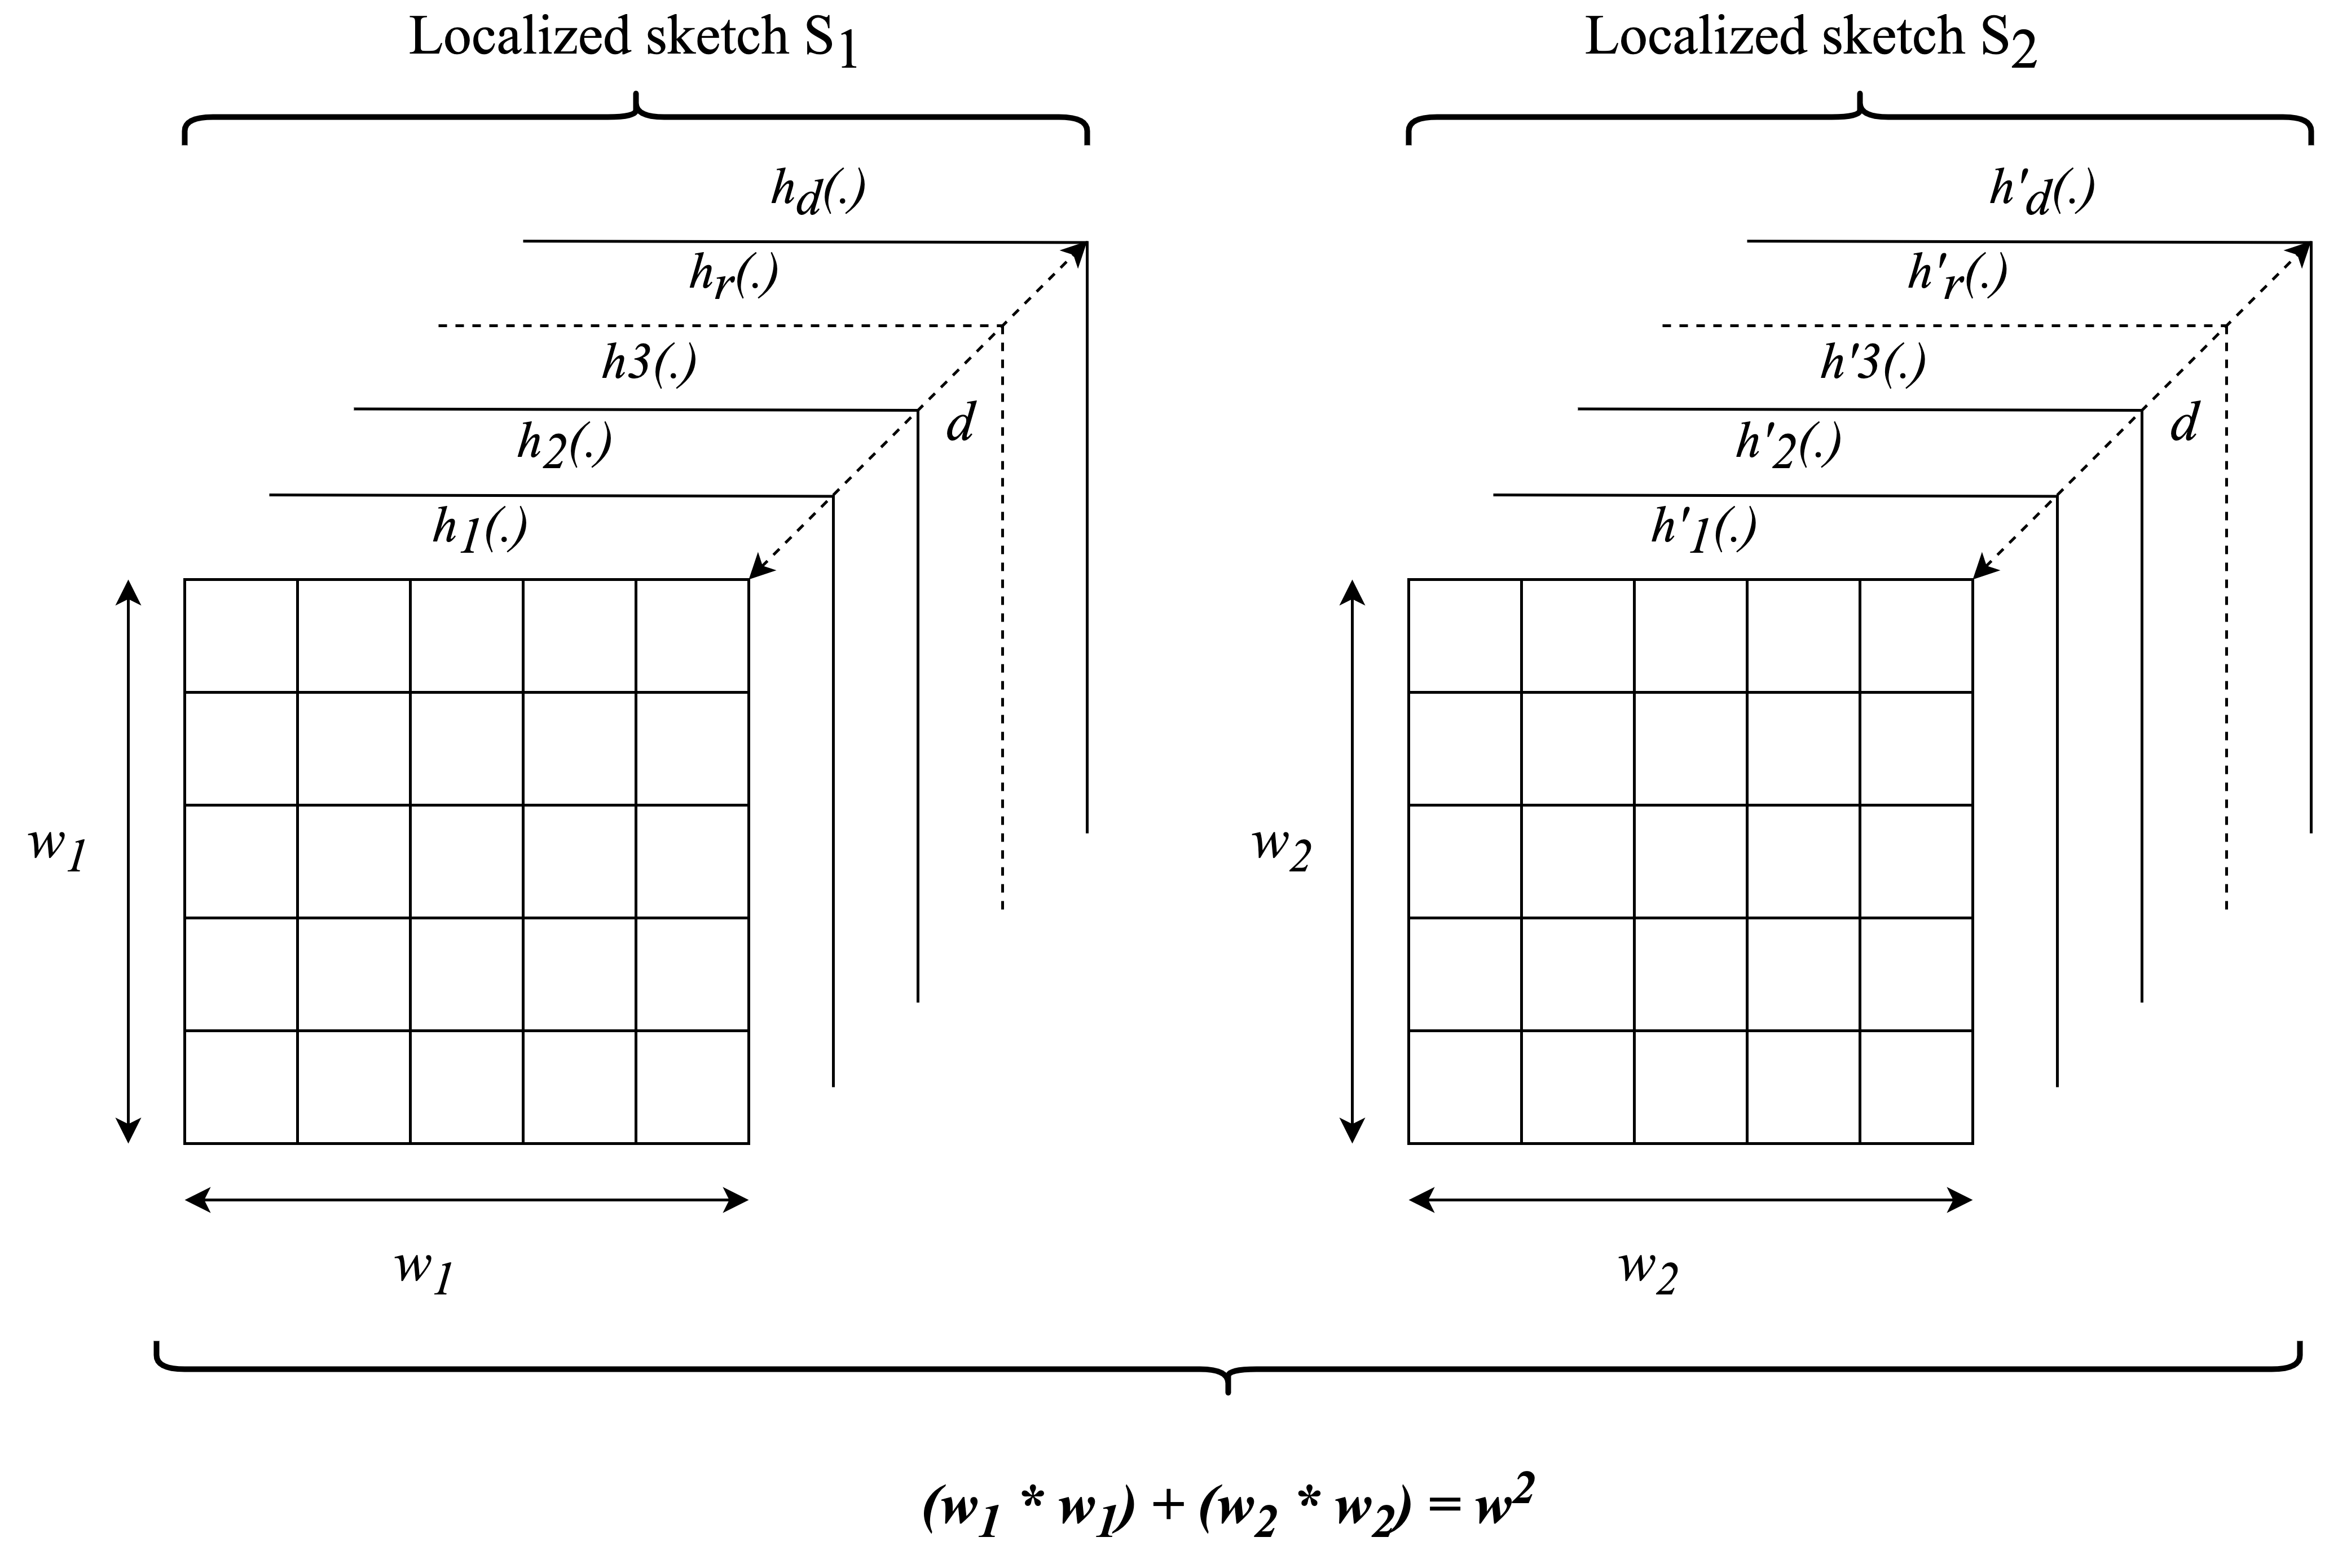
\includegraphics[width=\textwidth]{alpha}
    \caption{High level concept of Alpha sketch}
    \label{fig:alpha}
\end{figure}

\paragraph{}
The implementation code for alpha can be found in the appendix \autoref{appendix:alpha}.

\subsection{Partitioning algorithm in gSketch\cite{zhao_gsketch:_2011}}
\label{section:gsketch_partitioning}

\paragraph{}
A summarized version of the underlying theory and the algorithm is discussed in this section. The complete sketch partitioning process is given in the original gSketch paper.

\paragraph{}
Consider that the original sketch is partitioned into i sub-sketches. Let \(F(S_i)\) is the sum of the edge frequencies in the \(i\)th sketch. If \((m,n)\) is an edge in the \(i\)th sketch, let \(\bar{f}(m,n)\) be its expected frequency. Then,

\[\bar{f}(m,n) = (F(S_i) - f(m,n)) / w_i\]

\paragraph{}
Then the expected relative error of \((m,n)\) is given by,

\begin{equation}
    \bar{e}(m,n) = \bar{f}(m,n) / f(m,n) = F(S_i) / (f(m,n) . w_i) - 1 / w_i
    \label{eq:1}
\end{equation}

\paragraph{}
Then the overall relative error \(E_i\) of the sketch can be expressed as,

\begin{equation}
    \sum_{(m,n) \in S_i}^{} \bar{e}(m,n)
    \label{eq:2}
\end{equation}

\paragraph{}
Let the average frequency of a vertex be \(\tilde{f}_v(m)\) and the estimated out-degree of the \(m\) be \(\tilde{d}(m)\). Then the average frequency of the vertex would be \( \tilde{f}_v(m) / \tilde{d}(m) \). And the total estimated frequencies of the partitioned sketch \(S_i\) can be expressed as,

\begin{equation}
    \tilde{F}(S_i) = \sum_{m \in S_i \: ; \: m \in V}^{} \tilde{f}_v(m)
    \label{eq:3}
\end{equation}

\paragraph{}
According to the \autoref{eq:1}, \autoref{eq:2} and \autoref{eq:3},

\begin{equation}
    E_i = \sum_{m \in S_i}^{} \frac{\tilde{d}(m) . \tilde{F}(S_i)}{w_i . (\tilde{f}_v(m) / \tilde{d}(m))} - \sum_{m \in S_i}^{} \tilde{d}(m) / w_i
    \label{eq:4}
\end{equation}

\paragraph{}
\(\tilde{d}(m)\) in the numerator accounts for the fact that \(O(\tilde{d}(m))\) edges are coming out of the vertex m.

\paragraph{}
When a sketch of width \(w\) is partitioned into two sketches of widths \(w_1\) and \(w_2\), the total error can be expressed as \(E = E_1 + E_2\). Here \(w_1 = w_2\).

\begin{equation}
    E = \sum_{m \in S_1}^{} \frac{\tilde{d}(m) . \tilde{F}(S_i)}{w_1 . (\tilde{f}_v(m) / \tilde{d}(m))} + \sum_{m \in S_2}^{} \frac{\tilde{d}(m) . \tilde{F}(S_i)}{w_2 . (\tilde{f}_v(m) / \tilde{d}(m))} - \sum_{m \in S_1 \cup S_2}^{} \tilde{d}(m) / w_1
    \label{eq:5}
\end{equation}

\paragraph{}
The \autoref{eq:5} can be further simplified as,

\begin{equation}
    E' = E . w_1 + \sum_{m \in S_1 \cup S_2}^{} \tilde{d}(m)
\end{equation}

\paragraph{}
Here the value of \(E'\) is,

\begin{equation}
    E' = \sum_{m \in S_1}^{} \frac{\tilde{d}(m) . \tilde{F}(S_i)}{\tilde{f}_v(m) / \tilde{d}(m)} + \sum_{m \in S_2}^{} \frac{\tilde{d}(m) . \tilde{F}(S_i)}{\tilde{f}_v(m) / \tilde{d}(m)}
    \label{eq:6}
\end{equation}

\paragraph{}
So it is evident that the overall error can be minimized by choosing the smallest \(E'\) according to the \autoref{eq:6}. Therefor the underlying idea behind the partitioning algorithm is to choose a data sample of the original stream and then repeatedly partition the available space between the vertices in the sample according to the \autoref{eq:6}. After this initialization phase, the streaming can begin and the edges that represented the vertices in the sample got to their respective partitioned sketches.